\documentclass[hidelinks]{article}
\usepackage[a4paper, total={7in, 10in}]{geometry}
\usepackage[dvipsnames]{xcolor}
\usepackage{amsmath}
\usepackage{tikz}
\usepackage{tkz-euclide}
\usepackage[unicode]{hyperref}
\usepackage[all]{hypcap}
\usepackage{fancyhdr}
\usepackage{tocloft} % Add this package
\usepackage{xcolor}
\definecolor{darkgreen}{RGB}{0,100,0}
\usepackage{listings}
\lstset{
  language=R,
  basicstyle=\ttfamily\small,
  keywordstyle=\color{red},
  commentstyle=\color{darkgreen},
  stringstyle=\color{darkgreen},
  numbers=left,
  numberstyle=\tiny,
  stepnumber=1,
  numbersep=5pt,
  frame=single,
  breaklines=true,
  showstringspaces=false
}
\usepackage{amsmath}
\usepackage{amssymb}
\usepackage{pgfplots}
\pgfplotsset{compat=1.18}
\usepackage{amsmath}
\usepackage{float}
\usepackage{amsthm}
\usepackage[shortlabels]{enumitem}



% Remove dots from table of contents
\renewcommand{\cftdot}{}
\renewcommand{\cftsecdotsep}{\cftnodots}
\renewcommand{\cftsubsecdotsep}{\cftnodots}
\newcommand{\RNum}[1]{\uppercase\expandafter{\romannumeral #1\relax}}


\renewcommand{\contentsname}{Table of Contents}
\usetikzlibrary{angles,calc, decorations.pathreplacing}
\definecolor{carminered}{rgb}{1.0, 0.0, 0.22}
\definecolor{capri}{rgb}{0.0, 0.75, 1.0}
\definecolor{brightlavender}{rgb}{0.75, 0.58, 0.89}

\title{\textbf{STAT 545 HW 3}}
\author{Andres Efren Rocha Jayasinha}
\setcounter{secnumdepth}{0}
\date{Updated: \today} % suppresses the printed date

\begin{document}
\hypersetup{bookmarksnumbered=true,}
\pagecolor{white}
\color{black}
\maketitle
\begin{Large}
\tableofcontents
\end{Large}%
\pagebreak

\section{Assignment 3: Recurrence, Transience, and Periodicity}

\subsection{Exercise 3.23}

Consider a $k$-state Markov chain with transition matrix
\[
P =
\begin{pmatrix}
\frac{1}{k} & \frac{1}{k} & \frac{1}{k} & \cdots & \frac{1}{k} & \frac{1}{k} & \frac{1}{k} \\
1 & 0 & 0 & \cdots & 0 & 0 & 0 \\
0 & 1 & 0 & \cdots & 0 & 0 & 0 \\
\vdots & \vdots & \vdots & \ddots & \vdots & \vdots & \vdots \\
0 & 0 & 0 & \cdots & 0 & 0 & 0 \\
0 & 0 & 0 & \cdots & 1 & 0 & 0 \\
0 & 0 & 0 & \cdots & 0 & 1 & 0
\end{pmatrix}.
\]


\noindent Show that the chain is ergodic and find the limiting distribution.

\smallskip

{\color{darkgreen}

\noindent \textbf{Accessible}

\noindent State $j$ is said to be \emph{accessible} from state $i$ if $P_{ij}^n > 0$ for some $n \ge 0$. 
That is, there is positive probability of reaching $j$ from $i$ in a finite number of steps.
}

{\noindent \color{darkgreen}

\noindent \textbf{Communicate}

\noindent States $i$ and $j$ \emph{communicate} if $i$ is accessible from $j$ and $j$ is accessible from $i$.
}

{\noindent \color{darkgreen}

\noindent \textbf{Communication Class}

\noindent A communication class is a subset of the state space such that every pair of states in the subset communicate with each other, and no state in the subset communicates with any state outside the subset.
}

\medskip

{\noindent \color{darkgreen}
\textbf{Irreducibility}

\noindent A Markov chain is called \emph{irreducible} if it has exactly one communication class. 
That is, all states communicate with each other.
}

\medskip

{\noindent \color{darkgreen}
\textbf{Ergodic Markov Chain}

\noindent A Markov chain is called \emph{ergodic} if it is irreducible, aperiodic, and all states have finite expected return times. 
For finite Markov chains, the finiteness of expected return times always holds. 
Thus, a finite Markov chain is ergodic if and only if it is irreducible and aperiodic.
}

\medskip

{\color{darkgreen}

\noindent \textbf{Ergodic Chains and Regular Matrices}

\noindent Assume that $P$ is the transition matrix of a finite Markov chain.
The Markov chain is ergodic if and only if $P$ is regular.
}

\medskip

{\noindent \color{darkgreen}
\textbf{Fundamental Limit Theorem for Ergodic Markov Chains}

\noindent Let $X_0, X_1, \dots$ be an ergodic Markov chain. There exists a unique, positive, stationary distribution $\pi$, which is the limiting distribution of the chain. That is,
\[
\pi_j = \lim_{n \to \infty} P_{ij}^n \quad \text{for all } i,j.
\]
}

\noindent \textbf{Solution}

\noindent Consider the $k$-state Markov chain with transition matrix $P$ given above.
Observe first that from state $1$, the chain moves to any state
$j \in \{1,\dots,k\}$ with probability $1/k > 0$. Thus, state $1$ has
positive probability of reaching every state in one step.

\smallskip

\noindent For states $i \ge 2$, the transition structure is deterministic:
\[
P(i,i-1) = 1 \quad \text{for } i=2,\dots,k,
\]
so from any state $i$ the chain reaches state $1$ in exactly $i-1$ steps
with probability $1$.

\smallskip

\noindent Fix any state $i \in \{1,\dots,k\}$. In $i-1$ steps, the chain reaches
state $1$, and from state $1$ it can move to any state $j$ in one
additional step with probability $1/k$. Hence, for all $j$,
\[
P^{\,i}(i,j) \ge \frac{1}{k} > 0.
\]

\noindent It follows that the $i$-th row of $P^{\,i}$ is strictly positive.
Letting $n = \max\{1,2,\dots,k\} = k$, we conclude that $P^n$ has all
entries strictly positive. Therefore, the chain is \emph{regular}.

\noindent To find the limiting distribution, we solve for the stationary distribution
$\pi = (\pi_1,\dots,\pi_k)$ satisfying
\[
\pi = \pi P, \qquad \sum_{j=1}^k \pi_j = 1.
\]

\noindent From the structure of the transition matrix, we write the balance equations.

\noindent For state $1$, probability flows in from state $1$ with probability $1/k$
and from state $2$ with probability $1$, giving
\[
\pi_1 = \frac{1}{k}\pi_1 + \pi_2.
\]

\noindent For states $j = 2,\dots,k-1$, probability flows in from state $1$ with
probability $1/k$ and from state $j+1$ with probability $1$, so
\[
\pi_j = \frac{1}{k}\pi_1 + \pi_{j+1}.
\]

\noindent For state $k$, probability flows in only from state $1$, yielding
\[
\pi_k = \frac{1}{k}\pi_1.
\]

\noindent Solving these equations recursively, we obtain
\[
\pi_k = \frac{1}{k}\pi_1,
\]
\[
\pi_{k-1} = \frac{1}{k}\pi_1 + \pi_k = \frac{2}{k}\pi_1,
\]
\[
\pi_{k-2} = \frac{1}{k}\pi_1 + \pi_{k-1} = \frac{3}{k}\pi_1,
\]
\noindent and in general,
\[
\pi_j = \frac{k-j+1}{k}\,\pi_1, \qquad j=2,\dots,k.
\]

\noindent Using the normalization condition,
\[
1 = \sum_{j=1}^k \pi_j
= \pi_1 + \sum_{j=2}^k \frac{k-j+1}{k}\pi_1
= \pi_1 + \frac{\pi_1}{k} \sum_{m=1}^{k-1} m.
\]
Since $\sum_{m=1}^{k-1} m = \frac{(k-1)k}{2}$, we have
\[
1 = \pi_1\left(1 + \frac{k-1}{2}\right)
= \pi_1 \frac{k+1}{2},
\]
and hence
\[
\pi_1 = \frac{2}{k+1}.
\]

\noindent Therefore, the stationary (and limiting) distribution is
\[
\boxed{
\pi_j = \frac{2}{k(k+1)}(k-j+1), \qquad j=1,\dots,k.
}
\]

\noindent Since the chain is ergodic, this stationary distribution is also the
limiting distribution.

\subsection{Exercise 3.29}

Consider a Markov chain with transition matrix
\[
P=\begin{array}{c}
\\[-1.2ex]
\end{array}
\left(
\begin{array}{ccccccc}
0.6 & 0.2 & 0   & 0   & 0.2 & 0   & 0\\
0   & 0   & 0   & 0   & 0   & 0.5 & 0.5\\
0   & 0   & 0.3 & 0.7 & 0   & 0   & 0\\
0   & 0.3 & 0.4 & 0.3 & 0   & 0   & 0\\
0   & 0   & 0   & 0   & 1   & 0   & 0\\
0   & 0.1 & 0   & 0   & 0   & 0   & 0.9\\
0   & 0.2 & 0   & 0   & 0   & 0.8 & 0
\end{array}
\right).
\]
Identify the communication classes. Classify the states as recurrent or transient, and determine the period of each state.

\smallskip

\noindent \textcolor{darkgreen}{
\noindent \textbf{Recurrent and Transient States}
}

\noindent \textcolor{darkgreen}{
State $j$ is said to be \emph{recurrent} if the Markov chain started in $j$
eventually revisits $j$. That is, $f_j = 1$.
}

\noindent \textcolor{darkgreen}{
State $j$ is said to be \emph{transient} if there is positive probability that
the Markov chain started in $j$ never returns to $j$. That is, $f_j < 1$.
}

\medskip

{\noindent \color{darkgreen}
\textbf{Recurrence, Transience}
}

{\color{darkgreen}
\begin{enumerate}
\item[(i)] State $j$ is recurrent if and only if
\[
\sum_{n=0}^{\infty} P^{n}_{jj} = \infty .
\]

\item[(ii)] State $j$ is transient if and only if
\[
\sum_{n=0}^{\infty} P^{n}_{jj} < \infty .
\]
\end{enumerate}
}

{\noindent \color{darkgreen}
\textbf{Recurrence and Transience are Class Properties}
}

{\noindent \color{darkgreen}
\emph{The states of a communication class are either all recurrent
or all transient.}
}

\medskip

{\color{darkgreen}
\noindent \textbf{Period}
}

{\color{darkgreen}
\noindent For a Markov chain with transition matrix $P$, the \emph{period} of state $i$,
denoted $d(i)$, is the greatest common divisor of the set of possible return
times to $i$. That is,
\[
d(i) = \gcd\{\, n > 0 : P^{n}_{ii} > 0 \,\}.
\]
}

{\color{darkgreen}
\noindent If $d(i) = 1$, state $i$ is said to be \emph{aperiodic}. If the set of return
times is empty, set $d(i) = +\infty$.
}

\medskip

{\color{darkgreen}
\noindent \textbf{Periodicity is a Class Property}
}

\medskip

{\color{darkgreen}
\noindent \emph{The states of a communication class all have the same period.}
}

\medskip

{\color{darkgreen} \noindent \textbf{Closed Communication Class}

\noindent A communication class is \emph{closed} if it consists of all recurrent states.
A finite communication class is \emph{closed} only if it consists of all recurrent states.
}

\smallskip

\noindent \textbf{Solution}

\smallskip

\noindent \textit{\textbf{Identifying Communication Classes}}

\noindent From the transition graph, the communication classes can be identified as follows.

\smallskip

\noindent State $a$ can transition to $a$, $b$, and $e$, but no other state has a path back to $a$. Hence, $a$ does not communicate with any other state, and forms the
singleton communication class $\{a\}$.

\smallskip

\noindent State $e$ satisfies $P_{ee} = 1$, so once the chain enters $e$ it remains there forever. Thus, $e$ only communicates with itself and forms the singleton communication class $\{e\}$.

\smallskip

\noindent States $b$, $f$, and $g$ all communicate with one another. In particular, $b \to f,g$, $f \to b,g$, and $g \to b,f$, and there are no transitions from this set to states outside the set that return back. Therefore, $\{b,f,g\}$ is a communication class.

\smallskip

\noindent States $c$ and $d$ communicate with each other since $c \to d$ and $d \to c$, and each can also return to itself with positive probability. Hence,
$\{c,d\}$ forms a communication class.

\medskip

\noindent \textit{\textbf{Classification of States}}

\noindent We classify states as recurrent or transient by using the fact that recurrence
and transience are \emph{class properties}.

\smallskip

\noindent From the previous part, the communication classes are
\[
\{a\}, \quad \{e\}, \quad \{b,f,g\}, \quad \{c,d\}.
\]

\noindent By Theorem, all states in a communication class are either all recurrent or
all transient. Thus, it suffices to classify each communication class.

\smallskip

\noindent A communication class is said to be \emph{closed} if there are no transitions
from states in the class to states outside the class. {\color{red}In a finite Markov chain,
every closed communication class is recurrent, and every non-closed
communication class is transient}.

\smallskip

\noindent The class $\{e\}$ is closed, since $P_{ee}=1$ and no transitions leave state $e$.
Hence, state $e$ is recurrent.

\smallskip

\noindent The class $\{b,f,g\}$ is also closed. Transitions among these states remain
within the set, and there are no transitions from $b$, $f$, or $g$ to any state
outside the class. Therefore, states $b$, $f$, and $g$ are recurrent.

\smallskip

\noindent The class $\{c,d\}$ is not closed, since state $d$ can transition to state $b$,
which lies outside the class, and there is no path from $\{b,f,g\}$ back to
$\{c,d\}$. Thus, states $c$ and $d$ are transient.

\smallskip

\noindent Finally, the class $\{a\}$ is not closed, since state $a$ can transition to
states $b$ and $e$, and no other state has a transition back to $a$. Hence,
state $a$ is transient.

\smallskip

\noindent In summary, the recurrent states are
\[
\{b,f,g,e\},
\]
and the transient states are
\[
\{a,c,d\}.
\]

\smallskip

\noindent \textbf{\textit{Identifying the Period}}

\noindent We now determine the period of each state.

\smallskip

\noindent Recall that the period of a state $i$ is defined by
\[
d(i) = \gcd\{\, n > 0 : P^n_{ii} > 0 \,\}.
\]
\noindent By Lemma, periodicity is a class property, so it suffices to determine the
period for each communication class.

\noindent The communication classes are
\[
\{a\}, \quad \{e\}, \quad \{b,f,g\}, \quad \{c,d\}.
\]

\paragraph{Class $\{a\}$:}
Since $P_{aa} = 0.6 > 0$, a return to state $a$ is possible in one step. Hence,
\[
d(a) = 1,
\]
and $a$ is aperiodic.

\paragraph{Class $\{e\}$:}
State $e$ is absorbing, with $P_{ee} = 1$. Thus, a return to $e$ is possible in one
step, and
\[
d(e) = 1.
\]
Therefore, $e$ is aperiodic.

\paragraph{Class $\{b,f,g\}$:}
From state $b$, a return is possible in two steps (e.g.\ $b \to f \to b$ or
$b \to g \to b$) and in three steps (e.g.\ $b \to f \to g \to b$). Hence,
\[
\gcd\{2,3\} = 1,
\]
and the period of this class is $1$. Thus, states $b$, $f$, and $g$ are aperiodic.

\paragraph{Class $\{c,d\}$:}
State $c$ can return to itself in one step since $P_{cc} = 0.3 > 0$, and also in two
steps via $c \to d \to c$. Therefore,
\[
\gcd\{1,2\} = 1,
\]
and the period of this class is $1$. Hence, states $c$ and $d$ are aperiodic.

\subsection{Exercise 3.52}

The board for a modified Snakes and Ladder game is shown in
Figure 3.18. The game is played with a tetrahedron (four-faced) die.
\begin{enumerate}
\item[(a)] Find the expected length of the game.
\item[(b)] Assume that the player is on square 6. Find the probability that they will
find themselves on square 3 before finishing the game.
\end{enumerate}

\begin{figure}[H]
    \centering
    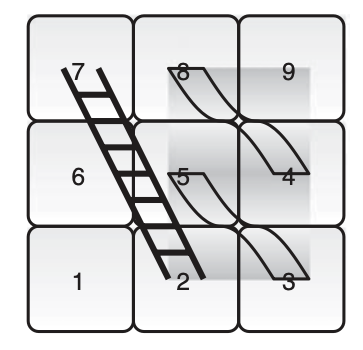
\includegraphics[width=0.2\linewidth]{figures/hw3-snakes-and-ladders-board.png}
    \caption{Figure 3.18 --- the modified Snakes and Ladders board.}
    \label{fig:snakes-and-ladders}
\end{figure}

\noindent \textbf{Solution}

\noindent Part A:

\noindent Expected length of the game.
Let the state space be $\{1,2,\dots,9\}$, with state $9$ absorbing (game over), and
let the transition matrix be
\[
P=\begin{pmatrix}
0 & 0 & \tfrac24 & \tfrac14 & 0 & 0 & \tfrac14 & 0 & 0\\
0 & 0 & \tfrac24 & \tfrac14 & 0 & \tfrac14 & 0 & 0 & 0\\
0 & 0 & \tfrac14 & \tfrac14 & 0 & \tfrac14 & \tfrac14 & 0 & 0\\
0 & 0 & \tfrac14 & \tfrac14 & 0 & \tfrac14 & \tfrac14 & 0 & 0\\
0 & 0 & 0 & \tfrac14 & 0 & \tfrac14 & \tfrac14 & 0 & \tfrac14\\
0 & 0 & 0 & \tfrac14 & 0 & 0 & \tfrac14 & 0 & \tfrac12\\
0 & 0 & 0 & \tfrac14 & 0 & 0 & 0 & 0 & \tfrac34\\
0 & 0 & 0 & 0 & 0 & 0 & 0 & 0 & 1\\
0 & 0 & 0 & 0 & 0 & 0 & 0 & 0 & 1
\end{pmatrix}.
\]

\noindent For $i=1,\dots,9$, define
\[
m_i := \mathbb{E}[\text{number of moves to reach state }9 \mid X_0=i].
\]
Clearly $m_9=0$. By first-step analysis, for each $i\neq 9$,
\[
m_i \;=\; 1 + \sum_{j=1}^9 P_{ij}\,m_j.
\]
Using the rows of the matrix $P$, this gives the system
\begin{align*}
m_1 &= 1 + \tfrac24 m_3 + \tfrac14 m_4 + \tfrac14 m_7,\\
m_2 &= 1 + \tfrac24 m_3 + \tfrac14 m_4 + \tfrac14 m_6,\\
m_3 &= 1 + \tfrac14 m_3 + \tfrac14 m_4 + \tfrac14 m_6 + \tfrac14 m_7,\\
m_4 &= 1 + \tfrac14 m_3 + \tfrac14 m_4 + \tfrac14 m_6 + \tfrac14 m_7,\\
m_5 &= 1 + \tfrac14 m_4 + \tfrac14 m_6 + \tfrac14 m_7 + \tfrac14 m_9,\\
m_6 &= 1 + \tfrac14 m_4 + \tfrac14 m_7 + \tfrac12 m_9,\\
m_7 &= 1 + \tfrac14 m_4 + \tfrac34 m_9,\\
m_8 &= 1 + m_9,\\
m_9 &= 0.
\end{align*}

\noindent Solving yields
\[
m_1=\frac{110}{23},\quad
m_2=\frac{113}{23},\quad
m_3=\frac{100}{23},\quad
m_4=\frac{100}{23},\quad
m_5=\frac{75}{23},\quad
m_6=\frac{60}{23},\quad
m_7=\frac{48}{23},\quad
m_8=1,\quad
m_9=0.
\]

\noindent \textit{Systems of Equations Calculator:} \href{https://matrixcalc.org/slu.html#solve-using-Gaussian-elimination%28%7B%7B-1,0,2/4,1/4,0,0,1/4,0,0,-1%7D,%7B0,-1,2/4,1/4,0,1/4,0,0,0,-1%7D,%7B0,0,-3/4,1/4,0,1/4,1/4,0,0,-1%7D,%7B0,0,1/4,-3/4,0,1/4,1/4,0,0,-1%7D,%7B0,0,0,1/4,-1,1/4,1/4,0,1/4,-1%7D,%7B0,0,0,1/4,0,-1,1/4,0,1/2,-1%7D,%7B0,0,0,1/4,0,0,-1,0,3/4,-1%7D,%7B0,0,0,0,0,0,0,-1,1,-1%7D,%7B0,0,0,0,0,0,0,0,1,0%7D%7D%29}{Solution Link}

\medskip

\noindent Therefore, starting from square $1$, the expected length of the game is
\[
\boxed{\mathbb{E}[\text{length of the game}\mid X_0=1]=m_1=\frac{110}{23}\approx 4.78\text{ moves}.}
\]

\noindent Part B:

\noindent Let
\[
h_i := \mathbb{P}_i(\text{hit state }3\text{ before hitting }9),
\]
i.e., the probability that starting from square $i$ the chain visits square $3$
before finishing the game (square $9$).

\noindent Then the boundary conditions are
\[
h_3 = 1,\qquad h_9 = 0.
\]
For $i\neq 3,9$, by first-step analysis,
\[
h_i \;=\; \sum_{j=1}^9 P_{ij}\,h_j.
\]

\noindent Using the transition matrix, we only need the equations for the
states accessible from $6$ before absorption:
\begin{align*}
h_7 &= \tfrac14 h_4 + \tfrac34 h_9,\\
h_6 &= \tfrac14 h_4 + \tfrac14 h_7 + \tfrac12 h_9,\\
h_4 &= \tfrac14 h_3 + \tfrac14 h_4 + \tfrac14 h_6 + \tfrac14 h_7.
\end{align*}
Substitute $h_3=1$ and $h_9=0$ to get
\[
h_7=\tfrac14 h_4,\qquad
h_6=\tfrac14 h_4+\tfrac14 h_7=\tfrac14 h_4+\tfrac1{16}h_4=\tfrac5{16}h_4.
\]
Plug these into the equation for $h_4$:
\[
h_4=\tfrac14+\tfrac14 h_4+\tfrac14\Big(\tfrac5{16}h_4\Big)+\tfrac14\Big(\tfrac14 h_4\Big)
=\tfrac14+\Big(\tfrac14+\tfrac5{64}+\tfrac1{16}\Big)h_4
=\tfrac14+\tfrac{25}{64}h_4.
\]
Hence
\[
\Big(1-\tfrac{25}{64}\Big)h_4=\tfrac14
\quad\Longrightarrow\quad
\tfrac{39}{64}h_4=\tfrac14
\quad\Longrightarrow\quad
h_4=\frac{16}{39}.
\]
Therefore
\[
h_6=\tfrac5{16}\,h_4=\tfrac5{16}\cdot \frac{16}{39}=\frac{5}{39}.
\]

\[
\boxed{\mathbb{P}_6(\text{hit }3\text{ before }9)=h_6=\frac{5}{39}.}
\]


\subsection{Exercise 3.54}

A mouse is placed in the maze in Figure~3.19 starting in
box $A$. A piece of cheese is put in box $I$. From each room the mouse moves to an
adjacent room through an open door, choosing from the available doors with equal
probability.
\begin{enumerate}
\item[(a)] How many rooms, on average, will the mouse visit before it finds the cheese?
\item[(b)] How many times, on average, will the mouse visit room $A$ before it finds
the cheese?
\end{enumerate}

\begin{figure}[H]
    \centering
    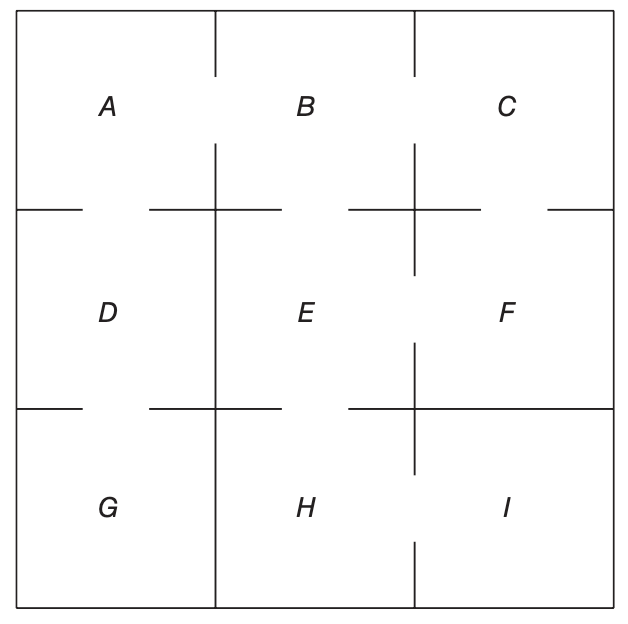
\includegraphics[width=0.16\linewidth]{figures/hw3-mouse-maze.png}
    \caption{Figure 3.19 --- the nine-room maze, with the mouse starting in $A$ and cheese in $I$.}
    \label{fig:mouse-maze}
\end{figure}

\noindent \textbf{Solution}

% States ordered as (A,B,C,D,E,F,G,H,I).
% From each room, the mouse chooses uniformly among the available open doors.
% Treat I as absorbing (once the cheese is found, the search ends).

\[
P=
\begin{array}{c}
\\[-1.2ex]
A\\ B\\ C\\ D\\ E\\ F\\ G\\ H\\ I
\end{array}
\left(
\begin{array}{ccccccccc}
A & B & C & D & E & F & G & H & I\\
0   & \tfrac12 & 0   & \tfrac12 & 0   & 0   & 0   & 0   & 0\\
\tfrac13 & 0   & \tfrac13 & 0   & \tfrac13 & 0   & 0   & 0   & 0\\
0   & \tfrac12 & 0   & 0   & 0   & \tfrac12 & 0   & 0   & 0\\
\tfrac12 & 0   & 0   & 0   & 0   & 0   & \tfrac12 & 0   & 0\\
0   & \tfrac13 & 0   & 0   & 0   & \tfrac13 & 0   & \tfrac13 & 0\\
0   & 0   & \tfrac12 & 0   & \tfrac12 & 0   & 0   & 0   & 0\\
0   & 0   & 0   & 1   & 0   & 0   & 0   & 0   & 0\\
0   & 0   & 0   & 0   & 1   & 0   & 0   & 0   & 0\\
0   & 0   & 0   & 0   & 0   & 0   & 0   & 0   & 1
\end{array}
\right).
\]

\noindent Part A:

\noindent Let $X_n$ denote the room occupied after the $n$th move, with state space
\[
\{A,B,C,D,E,F,G,H,I\},
\]
and let $I$ be the (absorbing) cheese room.  For each room $x$, define
\[
m_x := \mathbb{E}_x[T_I],
\qquad
T_I := \inf\{n\ge 0 : X_n = I\},
\]
so $m_x$ is the expected number of moves (equivalently, the expected number of
room-visits \emph{before} entering $I$) until the mouse finds the cheese when it
starts in room $x$.  Clearly $m_I = 0$.

\smallskip

\noindent From Figure~3.19, the open-door adjacencies are
\[
A\leftrightarrow B,\; A\leftrightarrow D,\;
B\leftrightarrow C,\; B\leftrightarrow E,\;
C\leftrightarrow F,\;
D\leftrightarrow G,\;
E\leftrightarrow F,\; E\leftrightarrow H,\;
H\leftrightarrow I,
\]
and from each room the mouse chooses uniformly among the available doors.
Thus the degrees are
\[
\deg(A)=2,\ \deg(B)=3,\ \deg(C)=2,\ \deg(D)=2,\ \deg(E)=3,\ \deg(F)=2,\ \deg(G)=1,\ \deg(H)=2.
\]

\noindent By first-step analysis, for each $x\neq I$,
\[
m_x \;=\; 1 + \sum_{y} P_{xy}\,m_y,
\]
which here yields the linear system
\begin{align*}
m_A &= 1 + \tfrac12 m_B + \tfrac12 m_D,\\
m_B &= 1 + \tfrac13(m_A+m_C+m_E),\\
m_C &= 1 + \tfrac12(m_B+m_F),\\
m_D &= 1 + \tfrac12(m_A+m_G),\\
m_E &= 1 + \tfrac13(m_B+m_F+m_H),\\
m_F &= 1 + \tfrac12(m_C+m_E),\\
m_G &= 1 + m_D,\\
m_H &= 1 + \tfrac12(m_E+m_I),\\
m_I &= 0.
\end{align*}
Solving gives
\[
m_A=\frac{89}{2},\quad
m_B=\frac{79}{2},\quad
m_C=39,\quad
m_D=\frac{95}{2},\quad
m_E=32,\quad
m_F=\frac{73}{2},\quad
m_G=\frac{97}{2},\quad
m_H=17,\quad
m_I=0.
\]
Therefore, starting from $A$, the expected number of rooms visited before the
mouse finds the cheese is
\[
\boxed{m_A=\frac{89}{2}=44.5.}
\]

\noindent Part B:

\noindent As in part (a), treat room $I$ as absorbing (once the mouse reaches $I$, the game
ends).  For each room $x\in\{A,B,C,D,E,F,G,H,I\}$ define
\[
v_x \;:=\; \mathbb{E}_x\!\left[\#\{\,n<T_I : X_n = A\,\}\right],
\qquad
T_I:=\inf\{n\ge 0: X_n=I\}.
\]
Thus $v_x$ is the expected number of \emph{visits to $A$} before the cheese is found,
starting from $x$.  In particular, the desired quantity is $v_A$.
(With this definition, the starting position counts as a visit, so starting in $A$
already contributes $1$.)

\noindent Clearly,
\[
v_I=0.
\]
By first-step analysis, for each $x\neq I$,
\[
v_x \;=\; \mathbf{1}\{x=A\} + \sum_y P_{xy}\,v_y,
\]
where $\mathbf{1}\{x=A\}=1$ if $x=A$ and $0$ otherwise.

\noindent Using the open-door transitions from Figure~3.19 (uniform among available doors),
we obtain the linear system
\begin{align*}
v_A &= 1 + \tfrac12 v_B + \tfrac12 v_D,\\
v_B &= \tfrac13(v_A+v_C+v_E),\\
v_C &= \tfrac12(v_B+v_F),\\
v_D &= \tfrac12(v_A+v_G),\\
v_E &= \tfrac13(v_B+v_F+v_H),\\
v_F &= \tfrac12(v_C+v_E),\\
v_G &= v_D,\\
v_H &= \tfrac12(v_E+v_I)=\tfrac12 v_E,\\
v_I &= 0.
\end{align*}

\noindent Solving yields
\[
v_A=\frac{15}{2},\quad
v_B=\frac{11}{2},\quad
v_C=5,\quad
v_D=\frac{15}{2},\quad
v_E=4,\quad
v_F=\frac{9}{2},\quad
v_G=\frac{15}{2},\quad
v_H=2,\quad
v_I=0.
\]

\textit{Sstems of Equation Calculator:}\href{https://matrixcalc.org/slu.html#solve-using-Gaussian-elimination%28%7B%7B-1,1/2,0,1/2,0,0,0,0,0,-1%7D,%7B1/3,-1,1/3,0,1/3,0,0,0,0,0%7D,%7B0,1/2,-1,0,0,1/2,0,0,0,0%7D,%7B1/2,0,0,-1,0,0,1/2,0,0,0%7D,%7B0,1/3,0,0,-1,1/3,0,1/3,0,0%7D,%7B0,0,1/2,0,1/2,-1,0,0,0,0%7D,%7B0,0,0,1,0,0,-1,0,0,0%7D,%7B0,0,0,0,1/2,0,0,-1,1/2,0%7D,%7B0,0,0,0,0,0,0,0,-1,0%7D%7D%29}{Solution Link}

Therefore, starting from $A$, the expected number of visits to room $A$ before the
mouse finds the cheese is
\[
\boxed{v_A=\frac{15}{2}=7.5.}
\]

\subsection{Exercise 3.66}

\textbf{R:} Simulate the expected hitting time for the random walk on the hexagon in Exercise 3.19.

\smallskip

\noindent \textbf{Solution}

\noindent \textbf{Input:}

\begin{lstlisting}[caption={Monte Carlo Simulation}]
# Random walk on the graph in Figure 3.15
# Estimate E_a[T_d] = expected hitting time to reach d starting from a

set.seed(123)

# --- Graph (neighbors) read from the figure ---
# Edges: a-b, b-c, c-d, d-e, e-f, f-a plus chords a-c, a-e, c-e
neighbors <- list(
  a = c("b","f","c","e"),
  b = c("a","c"),
  c = c("b","d","a","e"),
  d = c("c","e"),
  e = c("d","f","a","c"),
  f = c("a","e")
)

rw_hitting_time <- function(start = "a", target = "d", neighbors) {
  state <- start
  t <- 0L
  while (state != target) {
    state <- sample(neighbors[[state]], size = 1)
    t <- t + 1L
  }
  t
}

simulate_expected_hitting_time <- function(n_sims = 10000, start = "a", target = "d", neighbors) {
  times <- replicate(n_sims, rw_hitting_time(start, target, neighbors))
  list(
    estimate = mean(times),
    sd = sd(times),
    se = sd(times) / sqrt(n_sims),
    ci95 = mean(times) + c(-1, 1) * 1.96 * sd(times) / sqrt(n_sims)
  )
}

# --- Run the simulation ---
res <- simulate_expected_hitting_time(n_sims = 50000, start = "a", target = "d", neighbors = neighbors)
res
\end{lstlisting}


\noindent \textbf{Output:} 95\% Confidence Interval of (9.909, 10.059) where the units are steps. This matches up nicely with the exact value of 10 steps, which can be seen by solving the 3x3 linear system hinted in 3.19.


\end{document}